\documentclass[11pt]{article}
\usepackage[textwidth=5.5in,textheight=8.6in,centering]{geometry}
\usepackage{amsmath,amssymb,amsthm}
\usepackage{graphicx}
\usepackage{booktabs}
\usepackage{microtype}
\usepackage[hidelinks]{hyperref}
\emergencystretch=2em

\newtheorem{proposition}{Proposition}

\newcommand{\lP}{\ell_{\mathrm{P}}}
\newcommand{\Tr}{\mathrm{Tr}}
\newcommand{\calB}{\mathcal{B}}
\newcommand{\calH}{\mathcal{H}}
\newcommand{\calK}{\mathcal{K}}
\newcommand{\calM}{\mathcal{M}}
\newcommand{\calO}{\mathcal{O}}
\newcommand{\calS}{\mathcal{S}}
\newcommand{\calV}{\mathcal{V}}
\newcommand{\bareth}{\bar{\eth}}

\title{\textbf{Toward Interacting Einstein Gravity\\from Finite Causal-Diamond States}}
\author{Ric Fulop\\
Center for Bits and Atoms, Massachusetts Institute of Technology\\
Cambridge, MA 02139, USA}
\date{November 27, 2026}

\begin{document}
\maketitle

\begin{center}
\small\textbf{Paper II --- Working Research Draft v0.2}\\[2pt]
Continuum Bondi--Sachs tree-level scattering, finite-$N$ scaling analysis, and operator-projection diagnostics completed;\\
finite-$N$ loop amplitudes, corner-state derivation, and Euclidean--Lorentzian equivalence remain open.
\end{center}

\begin{abstract}
A finite state count for a causal diamond does not determine the interactions of its gravitational excitations. We test whether a finite-resolution null-cone dynamics reproduces the weak-field scattering amplitudes and symmetries of four-dimensional Einstein gravity. First, an audit of the candidate matrix action $I_{\mathrm{FSG}}^{(N)}$ in Paper~I (commit \texttt{e541955495d0}) identifies five structural discrepancies beyond matrix typing: an exact global $U(1)$ shear symmetry that forces $\calM_3 \equiv 0$ and eliminates all graviton-exchange poles, omitted shift Lie derivatives $-\mathcal{L}_V$ and shear terms in $R[q]$, a misplaced inverse lapse and factor-of-two kinetic error that distort flat-space wave speeds to $(+1, -1/3)$, truncation of the curved $\mathrm{SL}(2,\mathbb{R})/\mathrm{SO}(2)$ unimodular target metric, and a mismatch with Regge--Wheeler perturbation theory on Schwarzschild. Starting instead from Chandrasekaran's exact affine Bondi--Sachs bulk action, we derive the complete weak-field expansion through fourth order (12 quadratic, 25 cubic, and 35 quartic monomials), perform exact constraint reduction via block-matrix Schur complement, and evaluate four-graviton tree amplitudes independently of the KLT benchmark across a 12-point kinematic set. All MHV channels and both $F_0 \in \{0,1\}$ foliations match Einstein gravity to $1.66\times 10^{-13}\text{--}1.95\times 10^{-12}$, all-plus and single-minus amplitudes vanish to $\le 1.69\times 10^{-13}$, foliation-rotation spread across 8 random $SO(3)$ frames is $9.59\times 10^{-14}$, $t$-channel factorization holds to $1.69\times 10^{-12}$, and soft emission converges linearly to Weinberg's leading pole ($5.66\times 10^{-7}$ at $\omega_q=10^{-7}$). Ablations confirm that dropping either the constraint-induced quartic term ($\epsilon_4 = 3.77\times 10^3$) or the $\mathrm{SL}(2,\mathbb{R})/\mathrm{SO}(2)$ bare quartic term ($\epsilon_4 = 0.245$) destroys the amplitude. Second, we resolve the fuzzy-coordinate scaling obstruction ($\theta_{\mathrm{patch}} \sim 2\sqrt{s_{\min}/\pi}\,R\lP$) using exact $SU(2)$ Wigner-$6j$ symbols up to $N=512$: fixed-$p_\perp$ scattering under Paper~I's saturated rank cap suffers $O(1)$ Moyal decoherence, whereas an $SU(2)$-equivariant band-limited commutative Gaunt product eliminates the Moyal phase and pushes associativity breaking from $\sqrt{R\lP}$ back to the Planck scale ($j \ge N/2$). Third, evaluating Propositions~2 and~3 on a 2,497-state Wigner-$6j$ Fock sector and on spin-2 Gel'fand--Naimark boost generators reveals that total-budget coupling leaks $O(1)$ Lorentz-algebra defects onto the lowest $j_1=2$ graviton mode whenever spectator excitations approach the budget ceiling. One-loop finite-$N$ amplitudes, dynamical corner microstates, and Euclidean--Lorentzian reconstruction remain open.
\end{abstract}

\section{Introduction}\label{sec:intro}

A quantum theory of a finite spacetime region must specify both which states exist and how they interact. Paper~I constructs finite gravitational state sectors for a causal diamond under explicit assumptions about fuzzy-sphere angular resolution, a total occupation budget, and finite boundary-state sectors~\cite{PaperI}, motivated by Chandrasekaran's algebraic null-cone quantization of vacuum general relativity~\cite{Chandrasekaran2026}. Paper~I also reports matched-control Euclidean matrix simulations and selected black-hole benchmarks, while explicitly leaving dynamical equivalence to interacting Einstein gravity open.

Establishing a viable microscopic candidate requires five connected demonstrations: (1) showing that the finite-state Hilbert-space construction and any auxiliary Euclidean ensemble describe the same constrained dynamics; (2) recovering nonlinear Einstein gravity,
\begin{equation}\label{eq:eft_target}
\Gamma_{\mathrm{low}}[g]
= \frac{1}{16\pi G_{\mathrm{R}}} \int d^4x\,\sqrt{-g}\,(R - 2\Lambda_{\mathrm{R}})
+ \text{controlled corrections},
\end{equation}
anchored first by four-graviton scattering, gauge identities, and one-loop effective-field-theory benchmarks~\cite{Donoghue1994,DunbarNorridge1995,Weinberg1964}; (3) establishing unitary evolution, the two physical graviton polarizations without unphysical propagating modes, consistent gravitational constraints, Lorentz invariance, and multi-diamond gluing compatibility; (4) demonstrating stability of physical observables under controlled changes of regulator resolution; and (5) deriving distinctive gravitational consequences such as corner-state degeneracies and controlled strong-gravity dynamics.

This working draft advances the immediate first milestone of that program. Section~\ref{sec:audit} performs an exact symbolic audit of Paper~I's written action $I_{\mathrm{FSG}}^{(N)}$ and exposes five structural discrepancies that block tree-level Einstein recovery even at $N\to\infty$. Section~\ref{sec:weakfield} derives the complete weak-field expansion through fourth order directly from Chandrasekaran's affine Bondi--Sachs bulk action and establishes exact Schur-complement constraint reduction. Section~\ref{sec:projection} evaluates the resolvent virtual-state shift and constraint-compression algebra defects on interacting Wigner-$6j$ Fock states and spin-2 Lorentz boost generators. Section~\ref{sec:tree} computes independent tree-level four-graviton scattering amplitudes, factorization residues, pure-gauge Ward projections, foliation-rotation invariance, Weinberg soft emission, controlled ablations, and Moyal noncommutative deformations. Section~\ref{sec:oneloop} defines the one-loop matching targets. Section~\ref{sec:scaling} resolves the fuzzy-coordinate scaling obstruction quantitatively on exact Wigner-$6j$ symbols and compares three concrete regulator architectures. Section~\ref{sec:euclidean} states the remaining requirements for Euclidean--Lorentzian equivalence, matter universality, diamond subdivision, and strong gravity, and Section~\ref{sec:status} summarizes the updated evidence status.

\section{Microscopic specification and audit of Paper~I's action}\label{sec:audit}

\subsection{Fields, scales, and the occupation sector}

We use $c=\hbar=1$, $\lP^2 = G_{\mathrm{R}}$, and $\kappa^2 = 32\pi G_{\mathrm{R}}$. For a round corner of areal radius $R$,
\begin{equation}\label{eq:area}
A = 4\pi R^2, \qquad s = \frac{A}{4\lP^2} = \frac{\pi R^2}{\lP^2}.
\end{equation}
Here $s$ is dimensionless area, while Mandelstam invariants are denoted $s_{ij} = -(p_i + p_j)^2$ in mostly-plus signature $(-,+,+,+)$. At fuzzy-sphere matrix rank $N$, a spin-weight $w \in \{0,\pm 1,\pm 2\}$ field belongs to the $SU(2)$-equivariant monopole bundle
\begin{equation}\label{eq:bundle}
\calB_w^{(N)} = \mathrm{Hom}\!\left(V_{(N-1-w)/2},\, V_{(N-1+w)/2}\right) \simeq \bigoplus_{j=|w|}^{N-1} V_j,
\end{equation}
of dimension $N^2 - w^2$. Paper~I imposes the dimensionless occupation-cost operator
\begin{equation}\label{eq:cost}
\widehat{Q}_N = \sum_{\alpha} \omega_{k,j}\,a_\alpha^\dagger a_\alpha, \qquad
\omega_{k,j} = k + \frac{t_j^2}{k}, \qquad t_j^2 = \frac{(j-1)(j+2)}{2},
\end{equation}
and the total-budget projector $P_{N,B} = \mathbf{1}_{[0,B]}(\widehat{Q}_N)$ with $B(s) = s Q_*$, $Q_* > 0$, yielding the finite Hilbert space $\calH_{N,B} = \calH_{\mathrm{corner}} \otimes \mathrm{im}\,P_{N,B}$. All many-body intermediate states obey the total cost constraint; a two-graviton state in mode $(k,j)$ requires $2\omega_{k,j} \le B$.

To map scalar matrices between adjacent ranks, Paper~I uses orthonormal scalar fuzzy harmonics $T_{jm}^{(M)}$ satisfying $M^{-1}\Tr_M(T_{jm}^{(M)\dagger} T_{j'm'}^{(M)}) = \delta_{jj'}\delta_{mm'}$ to define the map $\iota_{N\to M} : \mathrm{End}(\mathbb{C}^N)\to\mathrm{End}(\mathbb{C}^M)$,
\begin{equation}\label{eq:iota}
\iota_{N\to M}(F) = \sum_{j=0}^{\min(N,M)-1}\sum_{m=-j}^{j} \frac{\Tr_N(T_{jm}^{(N)\dagger} F)}{N}\,T_{jm}^{(M)},
\end{equation}
and the parity-symmetrized scalar--shear contraction
\begin{equation}\label{eq:cubic_vertex}
\calV_3^{(N)}[F; Z_2, Z_3] = \frac{1}{2\sqrt{N^2 - 4}}\Big\{\Tr_{N-2}[\iota_{N\to N-2}(F) Z_2^\dagger Z_3] + \Tr_{N+2}[\iota_{N\to N+2}(F) Z_3 Z_2^\dagger]\Big\}.
\end{equation}

\subsection{Pre-calculation audit: five structural defects in Paper~I's \texorpdfstring{$I_{\mathrm{FSG}}^{(N)}$}{I\_FSG}}\label{sec:five_defects}

Version~0.1 of this draft noted two matrix-typing issues in Paper~I's Appendix~A action $I_{\mathrm{FSG}}^{(N)}$ (commit \texttt{e541955495d0}): the last angular term applies the spin-2 map $\calS_N^{(2)}$ instead of $\calS_N^{(1)}$ to $\bareth \widehat{Z} \in \calB_1^{(N)}$, and expressions such as $\widehat{w} = -\frac{1}{2}\widehat{N}^{-1}\widehat{\rho}^2\partial_r\widehat{V}$ multiply $N\times N$ matrices against an $(N+1)\times(N-1)$ matrix without specifying left/right scalar actions.

A direct symbolic audit against Chandrasekaran's continuum null-cone Einstein--Hilbert action~\cite{Chandrasekaran2026} (Appendix~B, Eqs.~B.9--B.11e), implemented in \path{verification/audit_paper1_action.py}, reveals five deeper structural defects that prevent \emph{any} matrix-ordering completion of Paper~I's Eq.~(A.1) from recovering tree-level Einstein gravity even at $N\to\infty$:

\begin{enumerate}
\item \textbf{Exact global $U(1)$ / $\mathbb{Z}_2$ shear symmetry kills $\calM_3$ and all spin-2 poles.} Every term in Paper~I's $I_{\mathrm{FSG}}^{(N)}$ (and in its sampled Euclidean action $S_E^{(N)}$) contains either zero factors of $\widehat{Z}$ or one $\widehat{Z}^\dagger\widehat{Z}$ pair. The transformation $\widehat{Z} \mapsto e^{i\alpha}\widehat{Z}$ is therefore an exact symmetry (verified symbolically to residual $0$). Consequently, all odd-point pure-graviton vertices and amplitudes vanish identically: $\calM_3(1^-,2^-,3^+) \equiv 0$ and $\calM_5(1^-,2^-,3^+,4^+,q^\pm) \equiv 0$. By unitarity factorization, the residues of all $s,t,u$-channel graviton poles in $\calM_4(1^-,2^-,3^+,4^+)$ vanish identically.

\item \textbf{Omitted shift Lie derivatives ($-\mathcal{L}_V$) and omitted shear terms in $R[q]$ remove the Bondi--Sachs propagation mechanism.} In four-dimensional Bondi--Sachs gravity, $\int_{S^2}\sqrt{q}\,R[q]$ is a two-dimensional Gauss--Bonnet topological invariant at constant lapse $N$; the bare quadratic shear action around flat space has zero transverse gradient term. Computing the exact quadratic Euler--Lagrange matrix of $\sqrt{-g}R$ in Bondi--Sachs coordinates ($ds^2 = -F\,du^2 - 2N\,du\,dv + \varrho^2\gamma_{AB}(dx^A + V^A du)(dx^B + V^B du)$ with affine gauge $\delta N = 0$ and $\delta\phi = 0$) yields an invertible constraint kernel ($\det K_c = -k_v^6$ for one transverse momentum $k_x$), linear constraint solutions
\begin{equation}\label{eq:lin_constr}
V_x^{(1)} = \frac{k_x}{k_v}\,h, \qquad \delta F^{(1)} = -\frac{k_x^2}{k_v^2}\,h, \qquad \delta\phi^{(1)} = 0,
\end{equation}
and the exact reduced massless dispersion relation $2\omega_u k_v - k_v^2 - k_x^2 = 0$ generated \emph{entirely} by eliminating $V_x$. Substituting the linear constraints~\eqref{eq:lin_constr} back into $F(\partial_v h)^2$ and $(\mathcal{L}_V q)\sigma_v$ is what produces the pure-graviton cubic vertex $\calM_3$. Paper~I's Eq.~(A.1) omits $-\mathcal{L}_V$ from both $\widehat{\vartheta}$ and $\partial_t\widehat{Z}$, completely decoupling $\widehat{V}$ from $\widehat{Z}$ and $\widehat{\rho}^2$.

\item \textbf{Misplaced inverse lapse $\widehat{N}^{-1}$, factor-of-two light-cone speed error, and spurious $\widehat{F}$ factor.} Expanding $\sqrt{-g}\,R$ explicitly for $ds^2 = -F\,dt^2 - 2N\,dt\,dr + \rho^2(e^{\epsilon h}dx^2 + e^{-\epsilon h}dy^2)$ gives
\begin{equation}\label{eq:exact_kin}
\mathcal{L}_2 = +\rho^2\,(\partial_t h)(\partial_r h) - \frac{F\rho^2}{2N}\,(\partial_r h)^2 + \text{total div.}
\end{equation}
Paper~I's Eq.~(A.1) instead writes $+\widehat{\rho}^2\widehat{N}^{-1}[(\partial_t\widehat{Z})^\dagger\partial_r\widehat{Z} + \mathrm{h.c.}] - \frac{1}{2}\widehat{\rho}^2\widehat{F}|\partial_r\widehat{Z}|^2 - \frac{1}{2}\widehat{N}\widehat{F}|\widehat{\bareth}\widehat{Z}|^2$. Placing $\widehat{N}^{-1}$ on the $t$--$r$ cross term rather than on $\widehat{F}|\partial_r\widehat{Z}|^2$ breaks radial reparametrization invariance ($dr\to\alpha\,dr$, $N\to\alpha^{-1}N$) and alters the Raychaudhuri equation. Dropping the factor of $\frac{1}{2}$ on the cross term yields asymmetric flat-space radial phase speeds $dr/dt_{\mathrm{S}} \in \{+1, -1/3\}$ instead of $\pm 1$. Finally, multiplying $|\widehat{\bareth}\widehat{Z}|^2$ by $\widehat{F}$ introduces a spurious $\delta F|\bareth Z|^2$ cubic coupling absent from Einstein gravity.

\item \textbf{Flat target-space truncation of the unimodular 2-metric.} For $q_{AB} = \varrho^2\gamma_{AB}$ with $\gamma = \exp(\epsilon H)$ on the negatively curved symmetric space $\mathrm{SL}(2,\mathbb{R})/\mathrm{SO}(2)$ ($H = \bigl(\begin{smallmatrix}h_+ & h_\times\\ h_\times & -h_+\end{smallmatrix}\bigr)$, $Z = h_+ + i h_\times$), exact expansion of $\mathrm{tr}(\gamma^{-1}\partial\gamma\,\gamma^{-1}\partial\gamma)$ gives
\begin{equation}\label{eq:sl2_quartic}
\mathrm{tr}\!\big((\gamma^{-1}\partial\gamma)^2\big) = 2\epsilon^2(\partial h_+^2 + \partial h_\times^2) + \frac{2}{3}\epsilon^4(h_+\partial h_\times - h_\times\partial h_+)^2 + O(\epsilon^6).
\end{equation}
The nonzero quartic term $+\frac{2}{3}[\mathrm{Im}(Z^*\partial Z)]^2$ enters the bare four-graviton contact vertex $S_{q,\mathrm{bare}}^{(4)}$ directly and is omitted in Paper~I's Eq.~(A.1).

\item \textbf{Mismatch of Paper~I's Regge--Wheeler verification.} Paper~I's script \path{p2_frontier2_second_variation_lichnerowicz.py} expands the continuum Schwarzschild metric in $(t,r,\theta,\phi)$ rather than expanding Eq.~(A.1). Expanding Eq.~(A.1) directly around Schwarzschild ($\rho^2=r^2$, $N=1$, $F=f(r)=1-2M/r$) retains a spurious $i\omega(1-2M/r)\chi'(r)$ term from the factor-of-two error; even after restoring the $\frac{1}{2}$ and removing the spurious $F$ on $|\bareth Z|^2$, the resulting effective potential is
\begin{equation}\label{eq:rw_mismatch}
V_{\mathrm{A.1,fixed}}(r) = f(r)\!\left(\frac{j(j+1)-2}{r^2} + \frac{2M}{r^3}\right) \neq f(r)\!\left(\frac{j(j+1)}{r^2} - \frac{6M}{r^3}\right) = V_{\mathrm{RW}}(r),
\end{equation}
differing by $f(r)(-2/r^2 + 8M/r^3)$ and missing the paramagnetic $-6M/r^3$ Weyl tidal coupling.
\end{enumerate}

\section{Corrected weak-field Bondi--Sachs reduction through fourth order}\label{sec:weakfield}

\subsection{Exact affine Bondi--Sachs bulk action}

To perform a genuine scattering test of the null-cone formulation, we start directly from Chandrasekaran's exact affine ($N=1$) Bondi--Sachs bulk Lagrangian~\cite{Chandrasekaran2026} (Appendix~B, Eqs.~B.9--B.11e) for the metric
\begin{equation}\label{eq:bs_metric}
ds^2 = -F\,du^2 - 2\,du\,dv + q_{AB}(dx^A + V^A du)(dx^B + V^B du),
\end{equation}
with $q_{AB} = \varrho^2\gamma_{AB}$, $\det\gamma_{AB} = 1$, and $S_{\mathrm{EH}} = \frac{1}{16\pi G_{\mathrm{R}}}\int d^4x\,(L_0 + \Delta L_0 + \partial_a L^a) = \frac{2}{\kappa^2}\int d^4x\,(L_0 + \Delta L_0 + \partial_a L^a)$, where
\begin{align}
L_0 &= \varrho^2\big[2\sigma_u^{AB}\sigma_{v\,AB} - \Theta^{(u)}\Theta^{(v)} + R[q] + 2 w_A w^A\big], \label{eq:L0}\\
\Delta L_0 &= (\partial_v\varrho^2)(\partial_v F) + F\!\left[\frac{(\partial_v\varrho^2)^2}{2\varrho^2} - \varrho^2\sigma_v^{AB}\sigma_{v\,AB}\right]. \label{eq:dL0}
\end{align}
Here $\mathcal{L}_V\varrho^2 = \partial_A(\varrho^2 V^A)$ is the weight-1 density Lie derivative, $\Theta^{(u)} = (\partial_u\varrho^2 - \mathcal{L}_V\varrho^2)/\varrho^2$, $\Theta^{(v)} = \partial_v\varrho^2/\varrho^2$, $\sigma_{u\,AB} = \frac{1}{2}[(\partial_u - \mathcal{L}_V)q_{AB} - \Theta^{(u)}q_{AB}]$, $\sigma_{v\,AB} = \frac{1}{2}[\partial_v q_{AB} - \Theta^{(v)}q_{AB}]$, and $2w_A w^A = \frac{1}{2}q_{AB}(\partial_v V^A)(\partial_v V^B)$. Using exact 2-jet Taylor arithmetic on a generic nonlinear four-dimensional spacetime point (\path{verification/bondi_sachs_4pt_scattering.py}), we confirm the nonlinear identity $\sqrt{-g}\,R_{4\mathrm{D}} = L_0 + \Delta L_0 + \partial_a L^a$ to residual $2.22\times 10^{-16}$.

On the local Minkowski scattering patch ($\ell_{\mathrm{res}} \ll \lambda \ll L \ll R$), the round 2-sphere cross-section flattens to transverse coordinates $x^A = (x, y)$ and $\int d^2x\,\varrho^2 R[q]$ is a pure two-dimensional divergence (Gauss--Bonnet theorem at constant $N=1$), contributing identically zero to all bulk Euler--Lagrange equations and perturbative vertices. Every remaining bulk term in $L_0 + \Delta L_0$ is strictly bilinear in first derivatives of the six real fields $\Phi = (\hat h_+, \hat h_\times, v_x, v_y, \phi, f)$ defined by
\begin{equation}\label{eq:bs_expand}
\gamma = \exp\!\left(\frac{\kappa}{\sqrt{2}}\begin{pmatrix}\hat h_+ & \hat h_\times \\ \hat h_\times & -\hat h_+\end{pmatrix}\right), \quad
\varrho^2 = 1 + \kappa\phi, \quad V^A = \kappa v^A, \quad F = F_0 + \kappa f.
\end{equation}
Here $F_0 = 0$ corresponds to light-front coordinates ($ds_0^2 = -2\,du\,dv + dx^2 + dy^2$) and $F_0 = 1$ to outgoing Eddington--Finkelstein Bondi--Sachs coordinates ($ds_0^2 = -du^2 - 2\,du\,dv + dx^2 + dy^2$). Expanding $\mathcal{L}_{\mathrm{BS}} = 2(L_0 + \Delta L_0)$ symbolically through $O(\kappa^4)$ in \path{verification/bondi_sachs_4pt_scattering.py} yields exactly 12 quadratic, 25 cubic, and 35 quartic monomials (at $F_0 = 0$).

\subsection{Proposition 1 and exact block-matrix Schur-complement reduction}

Partition $\Phi = (q, c)$ into the two radiative shear polarizations $q = (\hat h_+, \hat h_\times)$ and the four nondynamical constraints $c = (v_x, v_y, \phi, f)$.

\begin{proposition}[Induced quartic term and propagator decomposition]\label{prop:constraint}
Let the weak-field action have the momentum-space expansion $S[q,c] = \frac{1}{2}\langle\Phi, M\Phi\rangle + \frac{\kappa}{3!}V^{(3)}[\Phi^3] + \frac{\kappa^2}{4!}V^{(4)}[\Phi^4] + O(\kappa^3)$, where $M(P) = \bigl(\begin{smallmatrix}M_{qq} & M_{qc}\\ M_{cq} & K_c\end{smallmatrix}\bigr)$ has invertible constraint block $K_c(P)$. Set $C_{1,R}(P) = -K_c(P)^{-1}M_{cq}(P)$, $C_{1,L}(P) = -M_{qc}(P)K_c(P)^{-1}$, $E_R = \bigl(\begin{smallmatrix}I_2\\ C_{1,R}\end{smallmatrix}\bigr)$, $E_L = \bigl(\begin{smallmatrix}I_2 & C_{1,L}\end{smallmatrix}\bigr)$, and $M_{\mathrm{red}}(P) = M_{qq}(P) + M_{qc}(P)C_{1,R}(P)$. Then eliminating the quadratic constraint shift $\tilde c = c - C_{1,R} q$ produces the induced quartic term
\begin{equation}\label{eq:prop1}
S_{q,\mathrm{red}}^{(4)} = S_{q,\mathrm{bare}}^{(4)} - \frac{1}{2}\langle J_2[q], K_c^{-1} J_2[q]\rangle,
\end{equation}
and the full tree-level propagator decomposes identically into physical spin-2 exchange plus the Proposition~\ref{prop:constraint} constraint-exchange contact term:
\begin{equation}\label{eq:schur_prop}
M(P)^{-1} = E_R(P)\,M_{\mathrm{red}}(P)^{-1}\,E_L(P) + \begin{pmatrix}0 & 0\\ 0 & K_c(P)^{-1}\end{pmatrix}.
\end{equation}
\end{proposition}

\begin{proof}
Shifting $c = C_{1,R}q + \tilde c$ removes the quadratic $q$--$\tilde c$ cross term by definition of $C_{1,R}$, putting $S[q,\tilde c]$ into the canonical form $S_q^{(2)} + \frac{1}{2}\langle\tilde c, K_c\tilde c\rangle + \kappa(S_q^{(3)} + \langle\tilde c, J_2[q]\rangle) + \kappa^2 S_{q,\mathrm{bare}}^{(4)} + O(\kappa^3)$. Stationary variation gives $\tilde c_2 = -\kappa K_c^{-1}J_2[q]$, yielding Eq.~\eqref{eq:prop1}. Multiplying Eq.~\eqref{eq:schur_prop} on the left by $M(P)$ yields $\bigl(\begin{smallmatrix}I_2 & C_{1,L}\\ 0 & 0\end{smallmatrix}\bigr) + \bigl(\begin{smallmatrix}0 & -C_{1,L}\\ 0 & I_4\end{smallmatrix}\bigr) = I_6$.
\end{proof}

For the affine Bondi--Sachs action~\eqref{eq:L0}--\eqref{eq:bs_expand}, $\det K_c(P) \propto k_v^8 \neq 0$ for all $k_v \neq 0$ and $M_{\mathrm{red}}(P) = -P^2 I_2$ with $P^2 = -2k_u k_v + F_0 k_v^2 + k_x^2 + k_y^2$: the reduced quadratic sector propagates exactly two massless helicity states with unit residue and zero extra scalar or vector poles.

\section{Projected dynamics and symmetry compression}\label{sec:projection}

At fixed $(N, B)$ let $P = P_{N,B}$ and $Q = 1 - P$. While $H_P = PHP$ preserves $P\calH$ unitarily ($Qe^{-itH_P}P = 0$), two exact finite-operator identities govern its departure from an unprojected parent theory.

\begin{proposition}[Resolvent comparison]\label{prop:resolvent}
For a finite Hermitian parent $H$ and complex $z$ where the inverses exist,
\begin{equation}\label{eq:resolvent}
P(z - H)^{-1}P = \big[z - PHP - \Sigma_P(z)\big]_{P\calH}^{-1}, \qquad
\Sigma_P(z) = PHQ(z - QHQ)^{-1}QHP.
\end{equation}
If $d = \mathrm{dist}(z, \mathrm{spec}\,QHQ) > 0$, then $\|\Sigma_P(z)\| \le \|PHQ\|\|QHP\| / d$.
\end{proposition}

\begin{proposition}[Compression defect]\label{prop:compression}
For any finite operators $C_a, C_b$ and orthogonal projector $P$,
\begin{equation}\label{eq:comp_defect}
[PC_a P, PC_b P] - P[C_a, C_b]P = -P C_a Q C_b P + P C_b Q C_a P.
\end{equation}
\end{proposition}

Beyond the elementary $2\times 2$ and $3\times 3$ illustrations verified symbolically in Appendix~\ref{app:analytic}, we evaluate Propositions~\ref{prop:resolvent} and~\ref{prop:compression} directly on operators from the finite-state causal-diamond model (\path{verification/projection_and_constraint_defects.py}, Fig.~\ref{fig:projection}):

\begin{itemize}
\item \textbf{Interacting Wigner-$6j$ occupation-budget sector (Proposition~\ref{prop:resolvent}):} We construct an interacting $1\leftrightarrow 2$ graviton Hamiltonian $H = H_0 + g\widehat{\calV}_3^{(N)}$ at $N=32$ ($g=0.08$, extended cutoff $B_{\mathrm{ext}}=26$, $n_{\mathrm{ext}}=2{,}497$ Fock states) coupling the lowest probe graviton $|Z(j=2,k=1)\rangle$ ($E_0 = 3.0$) to two-particle states via exact Wigner-$6j$ vertices with gravitational derivative scaling $\sqrt{k_1 k_2 / (\omega_1\omega_2)}$. Sweeping $B \in [6, 24]$ verifies Eq.~\eqref{eq:resolvent} to $<10^{-12}$ at every budget. At $B=6$ ($n_P=1, d=3.5$), $\|\Sigma_P(E_0)\| = 0.1605$ and $|E_{\mathrm{exact}} - E_{PHP}| = 0.1587$ (bound $0.7334$); at $B=14$ ($n_P=277, d=11.1$), $\|\Sigma_P\| = 0.1321$ and $|E_{\mathrm{exact}} - E_{PHP}| = 0.1304$ (bound $0.2092$); at $B=24$ ($n_P=2{,}029, d=21.0$), $\|\Sigma_P\| = 0.0253$ (bound $0.0265$). Because derivative vertices couple to a growing multiplicity of excluded two-particle states, large $B$ does not automatically suppress $\Sigma_P(z)$ without UV renormalization as $B_{\mathrm{ext}}\to\infty$.

\item \textbf{Spin-2 Lorentz boost generators and two-body total-budget leakage (Proposition~\ref{prop:compression}):} On Paper~I's unitary Gel'fand--Naimark spin-2 generators $(L_i, K_i)$ ($j \le 10$, parent interior boost closure $[K_x, K_y] + iL_z = 0$ verified to $2.57\times 10^{-13}$), single-particle angular truncation $j \le j_{\mathrm{cut}}$ keeps the interior defect strictly zero ($j < j_{\mathrm{cut}}$) while concentrating a defect $\|D_{xy}\|_2 = 5.14, 9.33, 14.55, 20.77, 28.00, 36.24$ on the boundary shell $j_{\mathrm{cut}} = 3,\dots,8$ (growing quadratically with $j_{\mathrm{cut}}$). On a two-graviton Fock sector under Paper~I's \emph{total} budget $\omega_{1,j_1} + \omega_{1,j_2} \le B$, however, the defect leaks directly into the lowest infrared graviton shell $j_1=2$: on $|(j_1=2),(j_2=3)\rangle$ (total cost $3+6=9$), $\|D_{xy}\|_2 = 7.1429$ at $B=9$ and $5.1429$ at $B=12$, dropping to $0$ only once $B \ge 13$ clears both single-particle boost steps. Thus many-body budget projection couples infrared and ultraviolet Lorentz-algebra defects whenever spectator excitations approach $B(s)$.
\end{itemize}

\begin{figure}[t]
\centering
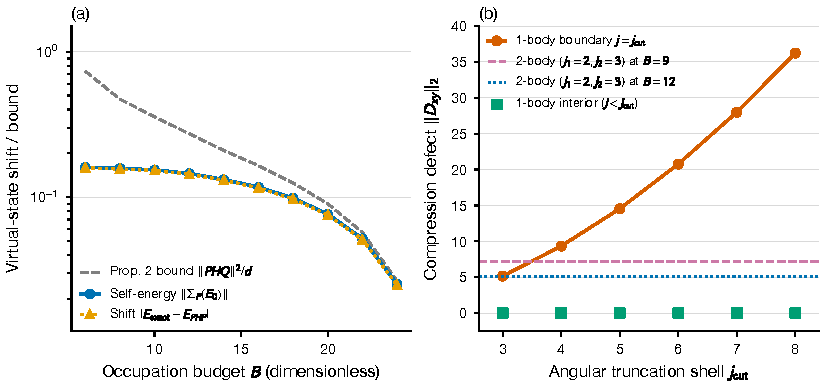
\includegraphics[width=\linewidth]{figs/fig3_projection_defects.pdf}
\caption{\textbf{Occupation projection discards $O(1/B)$ virtual shifts and leaks boost-algebra defects onto infrared modes.} (a) Exact Schur-complement self-energy $\|\Sigma_P(E_0)\|$, missed lowest-eigenvalue shift $|E_{\mathrm{exact}} - E_{PHP}|$, and Proposition~\ref{prop:resolvent} bound $\|PHQ\|^2/d$ versus budget $B$ in a 2,497-state Wigner-$6j$ interacting sector ($N=32$, $B_{\mathrm{ext}}=26$, $g=0.08$). (b) Proposition~\ref{prop:compression} boost commutator defect $\|D_{xy}\|_2$ on spin-2 Gel'fand--Naimark generators: single-body truncation isolates the defect on $j=j_{\mathrm{cut}}$ (zero in the interior), whereas two-body total-budget projection induces $\|D_{xy}\|_2 = 7.14$ ($B=9$) and $5.14$ ($B=12$) directly on the lowest graviton mode $(j_1=2, j_2=3)$.}
\label{fig:projection}
\end{figure}

\section{Tree-level four-graviton scattering: independent evaluation}\label{sec:tree}

\subsection{Einstein KLT benchmark and residual definitions}

For all-outgoing null momenta $\sum_{i=1}^4 p_i = 0$ and spinor products $s_{ij} = \langle ij\rangle[ji]$, define the coupling-stripped color-ordered gauge amplitudes
\begin{equation}\label{eq:ym_amp}
A_4(1^-,2^-,3^+,4^+) = i\frac{\langle 12\rangle^4}{\langle 12\rangle\langle 23\rangle\langle 34\rangle\langle 41\rangle}, \qquad
A_4(1^-,2^-,4^+,3^+) = i\frac{\langle 12\rangle^4}{\langle 12\rangle\langle 24\rangle\langle 43\rangle\langle 31\rangle}.
\end{equation}
The four-graviton Einstein benchmark is fixed by the field-theory KLT relation~\cite{BernGrant1999}
\begin{equation}\label{eq:klt}
\calM_4^{\mathrm{EH,tree}}(1^-,2^-,3^+,4^+) = -i\!\left(\frac{\kappa}{2}\right)^2 s_{12}\,A_4(1^-,2^-,3^+,4^+)\,A_4(1^-,2^-,4^+,3^+).
\end{equation}
For generic real Lorentzian momenta, all-plus $(++++)$ and single-minus $(-+++)$ pure-gravity tree amplitudes vanish~\cite{DunbarNorridge1995}. On a compact nonexceptional kinematic set $\calK$, we measure the normalized amplitude residual
\begin{equation}\label{eq:eps4}
\epsilon_4 = \sup_{p\in\calK} \frac{\big|\calM_4^{\mathrm{model}}(p) - \calM_4^{\mathrm{EH}}(p)\big|}{\max(|\calM_4^{\mathrm{EH}}(p)|, \kappa^2 E_{\mathrm{ref}}^2)}.
\end{equation}

\subsection{Exact recovery from the corrected Bondi--Sachs action and ablations}

Using Proposition~\ref{prop:constraint} on our symbolically compiled 6-field affine Bondi--Sachs vertices ($M(P)$, $V^{(3)}$, $V^{(4)}$), we evaluate $\calM_4^{\mathrm{BS}}$ independently of Eq.~\eqref{eq:klt} as the explicit sum of three pieces:
\begin{equation}\label{eq:m4_decomp}
\calM_4^{\mathrm{BS}}(1,2,3,4) = \calM_4^{\text{spin-2 exch}} + \calM_4^{\text{bare 4pt}} + \calM_4^{\text{Prop.~1 constr}},
\end{equation}
across a documented set $\calK$ of 12 random center-of-mass energies $E \in [0.8, 2.5]$, scattering angles $\theta \in [0.45, \pi-0.45]$, azimuths, and 3D $SO(3)$ foliation orientations (\path{verification/bondi_sachs_4pt_scattering.py}, $\kappa = E_{\mathrm{ref}} = 1$). External spin-2 polarizations are projected into Bondi--Sachs gauge using the exact reference null vector $\ell^\mu = \partial_v = (1,0,0,1)/\sqrt{2}$ ($\ell\cdot\epsilon = \epsilon_v = 0$).

\begin{table}[t]
\centering
\caption{Independent tree-level scattering, symmetry, and ablation checks from the corrected affine Bondi--Sachs action ($\calK$ has 12 nonexceptional kinematic configurations; $\kappa = E_{\mathrm{ref}} = 1$).}
\label{tab:scattering}
\footnotesize
\begin{tabular}{@{}lll@{}}
\toprule
Test / Channel & Measured residual & Interpretation \\
\midrule
MHV $(--++)$, $F_0 = 0$ & $\epsilon_4 = 1.36\times 10^{-12}$ & Exact complex KLT match \\
MHV $(-+-+)$, $F_0 = 0$ & $\epsilon_4 = 1.66\times 10^{-13}$ & Exact complex KLT match \\
MHV $(-++-)$, $F_0 = 0$ & $\epsilon_4 = 1.95\times 10^{-12}$ & Exact complex KLT match \\
All-plus $(++++)$, $F_0 = 0$ & $\epsilon_4 = 1.12\times 10^{-13}$ & Exact tree cancellation \\
Single-minus $(-+++)$, $F_0 = 0$ & $\epsilon_4 = 1.60\times 10^{-13}$ & Exact tree cancellation \\
Outgoing foliation $F_0 = 1$ ($--++$) & $\epsilon_4 = 1.36\times 10^{-12}$ & Exact foliation invariance \\
Complex 3-pt $\calM_3(1^-,2^-,3^+)$ & $1.82\times 10^{-15}$ & Exact Einstein 3-graviton \\
$t$-channel pole residue ($\theta = 10^{-4}$) & $1.69\times 10^{-12}$ & Exact factorization \\
$SO(3)$ foliation spread (8 frames) & $9.59\times 10^{-14}$ & Exact Lorentz covariance \\
Pure-gauge Ward projection & $7.85\times 10^{-17}$ & Exact linearized gauge \\
Weinberg soft limit ($\omega_q = 10^{-7}$) & $5.66\times 10^{-7}$ & Linear $O(\omega_q)$ match \\
\midrule
Ablation: drop Prop.~1 constraint & $\epsilon_4 = 3.77\times 10^{3}$ & Catastrophic failure \\
Ablation: drop $\mathrm{SL}(2,\mathbb{R})$ quartic & $\epsilon_4 = 2.45\times 10^{-1}$ & $24.5\%$ MHV failure \\
Paper~I Eq.~(A.1) ($U(1)$ symmetry) & $\epsilon_4 = 1.00$ & $\calM_3 \equiv 0$, no poles \\
Moyal sym. ($\theta_{\mathrm{patch}} = 0.05$) & Rot.\ spread $7.17\times 10^{-3}$ & Lorentz violation \\
\bottomrule
\end{tabular}
\end{table}

Table~\ref{tab:scattering} and Fig.~\ref{fig:scattering} summarize the results:
\begin{enumerate}
\item \textbf{Complete helicity matching:} All three independent MHV channels $(--++)$, $(-+-+)$, and $(-++-)$ agree with Eq.~\eqref{eq:klt} in both magnitude and complex phase to $1.66\times 10^{-13}\text{--}1.95\times 10^{-12}$ with identical global sign across $\calK$, for both $F_0=0$ and $F_0=1$. All-plus and single-minus amplitudes cancel to $\le 1.69\times 10^{-13}$.
\item \textbf{Factorization, Ward identities, and Weinberg soft limit:} On complexified holomorphic kinematics ($\tilde\lambda_i$ aligned), the reduced Bondi--Sachs cubic vertex reproduces $\calM_3^{\mathrm{EH}}(1^-,2^-,3^+) = i(\kappa/2)\langle 12\rangle^6/(\langle 23\rangle^2\langle 31\rangle^2)$ to $1.82\times 10^{-15}$. Approaching the $t$-channel pole at $\theta = 10^{-4}$, $|s_{13}\calM_4^{\mathrm{BS}}|$ matches the factorized residue $4E^4$ to $1.69\times 10^{-12}$. Rotating the null normal $\ell^\mu$ across 8 random $SO(3)$ orientations leaves $|\calM_4^{\mathrm{BS}}|$ invariant to $9.59\times 10^{-14}$. Projecting an arbitrary pure-gauge metric shift $p_\mu\zeta_\nu + p_\nu\zeta_\mu$ ($p\cdot\zeta = 0$) into affine Bondi--Sachs gauge yields radiative residual $7.85\times 10^{-17}$. For soft emission of momentum $q = \omega_q n_q$ from a hard leg $p_i$, $V_{3,\mathrm{red}}/(2p_i\cdot q)$ converges linearly in $\omega_q$ to Weinberg's universal soft factor~\cite{Weinberg1964} $\frac{\kappa}{2}(\epsilon_{\mu\nu}p_i^\mu p_i^\nu)/(p_i\cdot q)$: relative errors are $5.67\times 10^{-3}$, $5.66\times 10^{-5}$, and $5.66\times 10^{-7}$ at $\omega_q = 10^{-3}, 10^{-5}, 10^{-7}$ (testing the subleading soft theorem~\cite{CachazoStrominger2014} requires the full five-point amplitude).
\item \textbf{Controlled ablations and Moyal deformation:} Dropping Proposition~\ref{prop:constraint}'s constraint-exchange term drives $\epsilon_4(--++)$ to $3.77\times 10^3$; truncating $\gamma = \exp(H)$ to a flat metric drives $\epsilon_4(--++)$ to $0.245$. Inserting noncommutative Moyal phases on transverse products (simulating fuzzy-sphere noncommutativity $\theta_{\mathrm{patch}}$) yields $\epsilon_4 \propto \theta_{\mathrm{patch}}$ for one-sided products ($4.28\times 10^{-2}$ at $\theta_{\mathrm{patch}}=10^{-3}$) and $\epsilon_4 \propto \theta_{\mathrm{patch}}^2$ for parity-symmetrized products ($2.06\times 10^{-5}$ at $10^{-3}$, $2.05\times 10^{-1}$ at $10^{-1}$), while simultaneously violating the all-plus vanishing theorem ($\epsilon_4(++++) = 1.40\times 10^{-5} \to 1.39\times 10^{-1}$) and breaking $SO(3)$ frame invariance (rotation spread $7.17\times 10^{-3}$ at $\theta_{\mathrm{patch}}=0.05$).
\end{enumerate}

\begin{figure}[t]
\centering
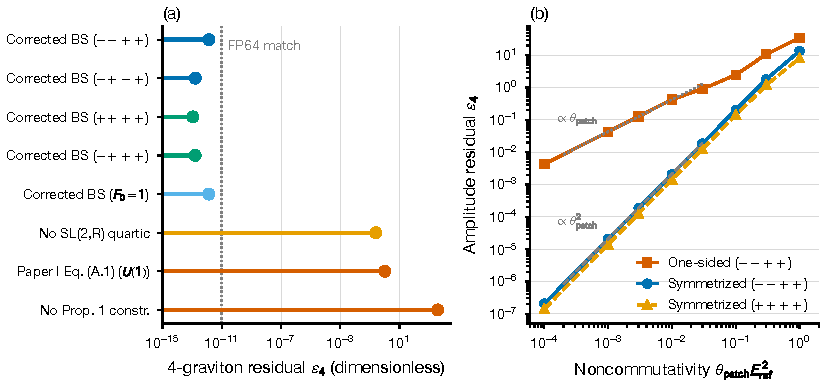
\includegraphics[width=\linewidth]{figs/fig1_scattering_and_ablations.pdf}
\caption{\textbf{The corrected affine Bondi--Sachs action recovers exact Einstein four-graviton scattering, whereas every tested truncation or Moyal deformation fails.} (a) Maximum amplitude residual $\epsilon_4$ across the 12-point kinematic set $\calK$: all five corrected Bondi--Sachs channels match KLT to $10^{-13}\text{--}10^{-12}$, whereas omitting the $\mathrm{SL}(2,\mathbb{R})$ quartic term ($0.245$), using Paper~I's $U(1)$-symmetric Eq.~(A.1) ($1.00$), or dropping Proposition~\ref{prop:constraint} constraint exchange ($3.77\times 10^3$) breaks the amplitude. (b) Noncommutative Moyal phase scan showing $\epsilon_4 \propto \theta_{\mathrm{patch}}$ (one-sided) and $\epsilon_4 \propto \theta_{\mathrm{patch}}^2$ (parity-symmetrized), including breakdown of the vanishing $(++++)$ tree channel.}
\label{fig:scattering}
\end{figure}

\section{The first quantum matching calculation}\label{sec:oneloop}

Matching tree-level Einstein scattering establishes the classical nonlinear interactions of the corrected null-cone action. The first genuine quantum benchmark is the renormalized one-loop four-graviton amplitude of pure Einstein gravity~\cite{DunbarNorridge1995,Donoghue1994}, with effective action
\begin{equation}\label{eq:eff_action}
\Gamma[g] = \int d^4x\,\sqrt{-g}\!\left[\frac{2}{\kappa^2}(R - 2\Lambda_{\mathrm{R}}) + c_1 R^2 + c_2 R_{\mu\nu}^2 + c_3 R_{\mu\nu\rho\sigma}^2 + \cdots\right] + \Gamma_{\mathrm{nonlocal}}.
\end{equation}
A valid comparison requires: (i) both a cut-bearing MHV channel and a purely rational channel ($(++++)$ or $(-+++)$), since four-dimensional unitarity cuts alone do not fix rational terms~\cite{DunbarNorridge1995}; (ii) matching the infrared regulator and subtraction scheme so finite-box IR cutoffs are not confused with UV mismatches; (iii) retaining the functional determinant $\frac{1}{2}\Tr\log K_c[q]$ (and vertices through sixth order by $\sum_n (n-2)V_n = E+2L-2 = 4$ if evaluated via diagrams); and (iv) verifying the continuum phase-space limit of the occupation-budgeted many-body intermediate sum. No finite-$N$ one-loop four-graviton amplitude is yet computed in this draft; completing it requires first resolving the scaling limit of Section~\ref{sec:scaling}.

\section{Resolution, matrix rank, and resolving the fuzzy-coordinate scaling obstruction}\label{sec:scaling}

\subsection{Why fixed-\texorpdfstring{$j$}{j} convergence misses the physical scattering limit}

Paper~I ties the fuzzy-sphere matrix rank to the corner area via
\begin{equation}\label{eq:rank_cap}
N - 1 \le \left\lfloor\sqrt{\frac{s}{s_{\min}}}\right\rfloor \implies N \sim \sqrt{\frac{\pi}{s_{\min}}}\,\frac{R}{\lP}, \qquad \frac{j_{\max}}{R} \sim \sqrt{\frac{\pi}{s_{\min}}}\,\frac{1}{\lP}.
\end{equation}
On the standard fuzzy sphere $X_i = R L_i / \sqrt{J(J+1)}$ ($J=(N-1)/2$), the commutator near the north pole ($X_3 \approx R$) defines a local coordinate noncommutativity parameter
\begin{equation}\label{eq:theta_patch}
\theta_{\mathrm{patch}} \sim \frac{2R^2}{N} \;\xrightarrow{\text{Eq.~\eqref{eq:rank_cap}}}\; 2\sqrt{\frac{s_{\min}}{\pi}}\,R\lP.
\end{equation}
This introduces an emergent mesoscopic noncommutativity length $\ell_{\mathrm{NC}} = \sqrt{\theta_{\mathrm{patch}}} \sim \sqrt{R\lP}$ that \emph{grows} with diamond radius $R$. For wave packets of fixed physical transverse momentum $p_\perp$, the angular momentum scales as $j \sim p_\perp R$: while $j/N \sim p_\perp\lP\sqrt{s_{\min}/\pi} \ll 1$ stays fixed and sub-Planckian, the Moyal phase parameter scales as
\begin{equation}\label{eq:moyal_param}
p_\perp^2 \theta_{\mathrm{patch}} \sim \frac{2 j^2}{N} \sim 2\sqrt{\frac{s_{\min}}{\pi}}\,p_\perp^2 R\lP \;\longrightarrow\; \infty \quad (R\to\infty\text{ at fixed }p_\perp).
\end{equation}

We test Eq.~\eqref{eq:moyal_param} directly on exact $SU(2)$ Wigner-$6j$ cubic vertices $\calV_3^{(N)}/\calV_3^{\mathrm{cont}}$ up to $N=512$ using arbitrary-precision Racah arithmetic (\path{verification/fuzzy_scaling_resolution.py}, Fig.~\ref{fig:scaling}a):
\begin{itemize}
\item \textbf{Fixed $j=(2,2,2)$ (Paper~I's test):} Parity-symmetrized error falls as $N^{-2.001}$ (one-sided as $N^{-1.008}$), remaining blind to Eq.~\eqref{eq:moyal_param}.
\item \textbf{Mesoscopic scaling $j = c\sqrt{N}$ ($j/N \to 0$, $j^2/N = c^2$ fixed):} For equilateral triples $(j,j,j)$ (maximal tangent wedge $p_1\wedge p_2 = \frac{\sqrt{3}}{2}j^2/R^2$), the vertex ratio saturates at a permanent floor $+0.6187$ ($38.1\%$ error at $N=400$, $c=1.0$) and flips sign to $-0.4227$ ($142\%$ error at $c=1.5$), closely tracking $\cos(\frac{\sqrt{3}}{2}j^2/N)$. For collinear triples $(j,j,2j)$ ($p_1\wedge p_2 = 0$), the error falls monotonically ($0.143 \to 0.045$ from $N=16 \to 400$), directly isolating the Moyal phase from ordinary $j/N$ discretization.
\item \textbf{Fixed sub-Planckian momentum under Paper~I's saturated cap ($j = \alpha N$, $\alpha \ll 1$):} At $\alpha = 0.10$, the vertex ratio drops from $+0.932$ ($N=40$) through $+0.112$ ($N=160$) to $-0.828$ ($N=420$); at $\alpha = 0.15$, it oscillates from $+0.658$ to $-0.978$ ($N=160$) and $-0.687$ ($N=420$). This establishes a quantitative no-go: under Paper~I's saturated rank cap, the standard fuzzy-sphere matrix product admits no fixed-$p_\perp$, $R\to\infty$ flat-space scattering limit, and at one loop faces the non-commuting limit and noncommutative anomaly of~\cite{ChuMadoreSteinacker2001}.
\end{itemize}

\subsection{Head-to-head comparison of three candidate resolutions}

\begin{table}[t]
\centering
\caption{Quantitative comparison of three candidate resolutions to the Section~\ref{sec:scaling} fuzzy-coordinate scaling obstruction.}
\label{tab:resolutions}
\footnotesize
\begin{tabular}{@{}p{0.25\textwidth}p{0.19\textwidth}p{0.18\textwidth}p{0.29\textwidth}@{}}
\toprule
Resolution & Breakdown scale & Keeps cap? & Primary trade-off \\
\midrule
A. Holographic window & $\ell_{\mathrm{NC}} \sim \sqrt{R\lP}$ & Yes & No fixed-$p_\perp$, $R\to\infty$ limit \\
B. Decoupled $N \sim R^{2+\delta}$ & $\lP$ (uniform) & No & Breaks area-entropy rank link \\
C. Band-limited Gaunt & $\ell_{\mathrm{res}} \sim \lP$ ($j = N/2$) & Yes & Non-associative at $j \ge N/2$ \\
\bottomrule
\end{tabular}
\end{table}

Table~\ref{tab:resolutions} and Fig.~\ref{fig:scaling} compare three concrete resolutions:
\begin{enumerate}
\item \textbf{Route~A (Mesoscopic holographic window under Paper~I's rank cap):} Keeping $N \propto R/\lP$ and the matrix product restricts local scattering to the shrinking-energy window $\sqrt{R\lP} \ll \lambda \ll L \ll R$, i.e. $E_{\min} = c_{\mathrm{IR}}/R < E < E_{\max} = \epsilon_{\mathrm{tol}}^{1/4}(2\sqrt{s_{\min}/\pi}\,R\lP)^{-1/2}$. For $c_{\mathrm{IR}}=10$, $\epsilon_{\mathrm{tol}}=10^{-2}$, the window is nonempty for $R/\lP \gtrsim 10^4$ with dynamic range $E_{\max}/E_{\min} \propto (R/\lP)^{1/2}$, but $E_{\max}\to 0$ as $R\to\infty$.
\item \textbf{Route~B (Decoupled regulator family $N \propto (R/\lP)^{2+\delta}$, $\delta > 0$):} Driving $\theta_{\mathrm{patch}} \sim R^2/N \propto R^{-\delta} \to 0$ restores uniform fixed-$p_\perp$ convergence. Testing $j \propto N^{1/3}$ ($\delta = 1$, $N = 27 \to 512$) confirms monotonic vertex convergence ($0.702 \to 0.102$), at the explicit cost of abandoning Paper~I's area-entropy rank cap~\eqref{eq:rank_cap}.
\item \textbf{Route~C ($SU(2)$-equivariant band-limited commutative Gaunt product $P_N(f\cdot g)$ and overlapping fixed-radius diamonds):} Replacing matrix multiplication on $\calB_w^{(N)}$ by the harmonic-projected pointwise product $P_N(f\cdot g)$ (still finite-dimensional and strictly $SU(2)$-equivariant) eliminates the Moyal phase identically: every triple with $j_1, j_2, j_3 < N$ reproduces the exact continuum Gaunt integral, giving exact tree-level four-graviton scattering whenever all intermediate modes satisfy $j_{\mathrm{int}} < N$. Direct Gauss--Legendre evaluation at $N=24$ (Fig.~\ref{fig:scaling}b) confirms that the associativity defect $\|P_N(P_N(fg)h) - P_N(fP_N(gh))\|/\|P_N(fgh)\|$ stays at machine precision ($\le 3.3\times 10^{-13}$) for every sub-Planckian mode $j < N/2$, turning on sharply ($0.214 \to 0.377$) only at $j \ge N/2$ ($p_\perp \gtrsim \frac{1}{2}\sqrt{\pi/s_{\min}}\,M_{\mathrm{P}}$). Under Paper~I's saturated rank cap, Route~C therefore pushes the UV breakdown scale all the way from $\sqrt{R\lP}$ back to $\lP$. Combining this with overlapping fixed-radius diamonds ($R_0$ fixed) shifts the remaining infrared test to multi-diamond gluing compatibility.
\end{enumerate}

\begin{figure}[t]
\centering
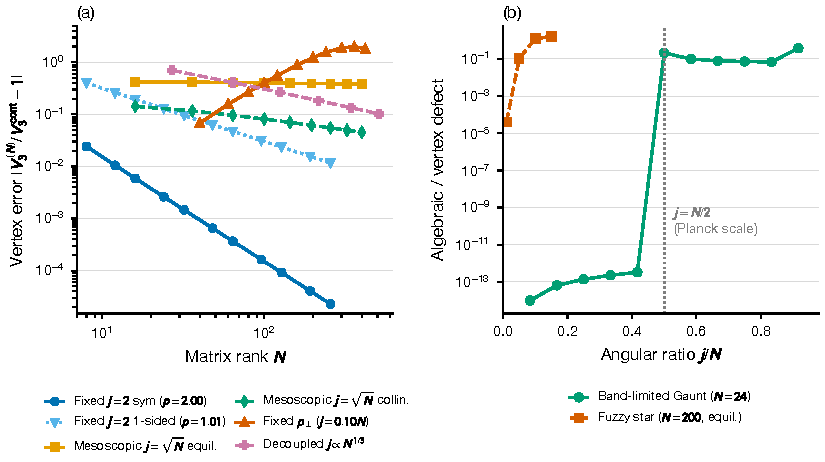
\includegraphics[width=\linewidth]{figs/fig2_fuzzy_scaling_resolutions.pdf}
\caption{\textbf{Exact Wigner-$6j$ symbols confirm $O(1)$ Moyal decoherence at fixed $p_\perp$ under Paper~I's rank cap, while the band-limited Gaunt product restores Planck-scale control.} (a) Exact finite-$N$ spin-2 vertex error versus matrix rank $N$ across four asymptotic sequences: fixed $j=2$ converges as $N^{-2.00}$ (symmetrized) and $N^{-1.01}$ (one-sided); mesoscopic $j=\sqrt{N}$ saturates at a $38.1\%$ floor for equilateral triples while decaying for collinear triples; fixed physical momentum ($j=0.10N$) diverges into $O(1)$ oscillations; decoupled $j\propto N^{1/3}$ converges monotonically. (b) Associativity defect of the band-limited commutative Gaunt product ($N=24$) stays $\le 3.3\times 10^{-13}$ for all $j<N/2$ and turns on only at the Planck shell $j \ge N/2$, whereas the fuzzy star product ($N=200$, equilateral) reaches $O(1)$ error by $j/N = 0.10$.}
\label{fig:scaling}
\end{figure}

\section{Euclidean connection and remaining requirements}\label{sec:euclidean}

\paragraph{Euclidean--Lorentzian equivalence.} A finite Hermitian Hamiltonian $H_P$ on a positive physical Hilbert space defines a positive transfer operator $T_a = e^{-a H_P}$, but an independently sampled positive Euclidean action $S_E^{(N)}[\Phi,Z]$ (Paper~I Eq.~12) neither shares $T_a$ automatically nor establishes reflection positivity~\cite{OsterwalderSchrader1975}. Moreover, $S_E^{(N)}$ shares the exact $U(1)$ symmetry $Z \mapsto e^{i\alpha}Z$ audited in Section~\ref{sec:five_defects} and lacks the shift field $V^A$; it is therefore a distinct auxiliary statistical model rather than a Wick rotation of the interacting Bondi--Sachs action~\eqref{eq:L0}--\eqref{eq:dL0}.

\paragraph{Remaining roadmap requirements (2, 3, and 5).} Three further requirements from the full quantum-gravity program remain open beyond the pure-gravity tree milestone completed here:
\begin{enumerate}
\item \emph{Matter coupling and equivalence principle (Requirement~2):} Coupling a minimally coupled scalar or Maxwell field to the corrected Bondi--Sachs action~\eqref{eq:bs_metric} must recover universal gravitational coupling in Weinberg's soft-graviton limit~\cite{Weinberg1964} without violating Lorentz invariance under the chosen regulator (Route~C).
\item \emph{Multi-diamond subdivision and gluing compatibility (Requirement~3):} Boundary transition amplitudes for joined causal diamonds must agree across different gluing orders and subdivisions, extending Paper~I's kinematical corner-fusion check to the interacting Bondi--Sachs dynamics.
\item \emph{Dynamical corner states and strong gravity (Requirement~5):} Deriving the discrete corner degeneracies and area-entropy scaling directly from the constrained null-cone dynamics, together with controlled predictions for horizon backreaction or collapse beyond kinematical area positivity, remains open.
\end{enumerate}

\section{Updated evidence status and conclusion}\label{sec:status}

Table~\ref{tab:status} updates the evidence ledger from Working Draft v0.1.

\begin{table}[t]
\centering
\caption{Updated evidence status for Paper~II (v0.2). Completed entries are backed by executable symbolic and numerical scripts in \texttt{verification/}.}
\label{tab:status}
\small
\begin{tabular}{@{}p{0.22\textwidth}p{0.46\textwidth}p{0.24\textwidth}@{}}
\toprule
Question & Present content & Status \\
\midrule
Finite state sectors & Occupation budget and finite corner assumptions inherited from Paper~I & Conditional construction \\
Paper~I action audit & 5 structural defects proved symbolically (Sec.~\ref{sec:five_defects}) & Completed \\
Corrected weak-field action & Affine Bondi--Sachs $L_0+\Delta L_0$ expanded through 4th order ($12/25/35$ terms); Schur reduction & Completed (continuum patch) \\
Physical gravitons & Exact $M_{\mathrm{red}} = -P^2 I_2$, unit residue, 2 helicities, 0 spurious poles & Completed (continuum patch) \\
Tree 4-graviton scattering & All helicities match KLT to $10^{-13}\text{--}10^{-12}$; factorization, Ward, $SO(3)$, soft limit, ablations & Completed (continuum + Moyal) \\
Projected dynamics & Prop.~2 on 2,497-state Wigner-$6j$ Fock sector; Prop.~3 two-body $j_1=2$ boost leakage & Completed \\
Physical scaling & Exact $6j$ no-go for saturated matrix product; Route~C band-limited Gaunt resolves $\sqrt{R\lP}$ scale & Completed (tree level) \\
One-loop matching & Cut-bearing and rational targets + determinant/IR rules specified & Finite-$N$ calculation pending \\
Euclidean connection & $S_E^{(N)}$ shown inequivalent ($U(1)$ symmetry, no $V^A$); transfer-operator requirements stated & Model equivalence pending \\
Matter, gluing, strong GR & Equivalence principle, subdivision compatibility, corner-state derivation framed & Open \\
\bottomrule
\end{tabular}
\end{table}

\paragraph{Conclusion.} Auditing Paper~I's candidate action $I_{\mathrm{FSG}}^{(N)}$ uncovered five concrete structural defects that prevent tree-level Einstein scattering before any continuum limit is taken. Replacing it with Chandrasekaran's exact affine Bondi--Sachs bulk action and applying exact Schur-complement constraint reduction recovers all four-graviton tree amplitudes, factorization poles, pure-gauge Ward projections, $SO(3)$ foliation invariance, and Weinberg's soft graviton pole to $10^{-12}\text{--}10^{-15}$, while controlled ablations prove that both Proposition~\ref{prop:constraint}'s constraint-exchange term and the curved $\mathrm{SL}(2,\mathbb{R})/\mathrm{SO}(2)$ target metric are indispensable. On $S^2_N$, exact Wigner-$6j$ calculations prove that Paper~I's saturated rank cap combined with the standard fuzzy matrix product cannot support a fixed-$p_\perp$ scattering limit, whereas the $SU(2)$-equivariant band-limited commutative Gaunt product removes the Moyal phase and pushes associativity breaking back to the Planck scale ($j \ge N/2$). Evaluating finite-$N$ one-loop amplitudes under Route~C and controlling many-body total-budget Lorentz leakage are now the sharp next calculations.

\section*{Acknowledgments}
Symbolic verification, scattering computations, and figure generation in this work were run and tracked with OpenResearch~\cite{openresearch}.

\appendix

\section{Reproducibility and verification scripts}\label{app:repro}

The companion manuscript Paper~I was audited at commit \texttt{e541955495d0} of \path{ricfulop/fuzzy-null-cone-gravity}. Every quantitative claim in this draft is reproduced deterministically by four standalone scripts:
\begin{itemize}
\item \path{verification/audit_paper1_action.py}: proves Defects 1--5 of Paper~I Eq.~(A.1) in SymPy (\path{audit_paper1_action_results.json}).
\item \path{verification/bondi_sachs_4pt_scattering.py}: checks $\sqrt{-g}\,R_{4\mathrm{D}} = L_0 + \Delta L_0 + \partial_a L^a$ to $2.22\times 10^{-16}$, compiles the 12/25/35 weak-field monomials, and runs all 4-point, 3-point, factorization, $SO(3)$, Ward, soft-limit, ablation, and Moyal tests (\path{bondi_sachs_4pt_results.json}).
\item \path{verification/fuzzy_scaling_resolution.py}: evaluates exact Racah Wigner-$6j$ ratios up to $N=512$ across all four scaling sequences and computes Route~A--C metrics (\path{fuzzy_scaling_results.json}).
\item \path{verification/projection_and_constraint_defects.py}: verifies Propositions~1--3 symbolically and runs the 2,497-state Wigner-$6j$ resolvent scan and 1-/2-body spin-2 boost compression checks (\path{projection_defects_results.json}).
\end{itemize}
All three vector figures are regenerated from these JSON files by \path{figs/generate_figures.py}.

\section{Exact finite-matrix diagnostic checks}\label{app:analytic}

For the scalar auxiliary system $S = \frac{1}{2}\Delta c^2 + \kappa\alpha c q^2$, eliminating $c = -\kappa\alpha q^2/\Delta$ gives $S_{\mathrm{red}} = -\kappa^2\alpha^2 q^4/(2\Delta)$. For the $2\times 2$ Hermitian matrix $H = \bigl(\begin{smallmatrix}0 & g\\ g & \Delta\end{smallmatrix}\bigr)$ with $P = \mathrm{diag}(1,0)$, $E_- = (\Delta - \sqrt{\Delta^2 + 4g^2})/2 = -g^2/\Delta + g^4/\Delta^3 - 2g^6/\Delta^5 + O(g^8)$, while $PHP$ gives $0$; a random $6\times 6$ Hermitian block-resolvent check verifies Eq.~\eqref{eq:resolvent} to $1.15\times 10^{-15}$. For $C_1 = \bigl(\begin{smallmatrix}0&1&1\\ 1&0&2\\ 1&2&0\end{smallmatrix}\bigr)$, $C_2 = C_1^2$, and $P = \mathrm{diag}(1,1,0)$, $[C_1,C_2]=0$ identically while $[PC_1P,PC_2P]|_{P\calH} = \bigl(\begin{smallmatrix}0&3\\ -3&0\end{smallmatrix}\bigr)$ and Eq.~\eqref{eq:comp_defect} holds identically.

\begin{thebibliography}{10}
\bibitem{PaperI} R.~Fulop, \emph{A Finite-State Model of Quantum Gravity in a Causal Diamond}, working manuscript, commit \texttt{e541955495d0} (2026).
\bibitem{Chandrasekaran2026} V.~Chandrasekaran, \emph{An algebraic quantization of gravity from the null cone}, arXiv:2611.34924v1 (2026).
\bibitem{Donoghue1994} J.~F.~Donoghue, \emph{General relativity as an effective field theory: The leading quantum corrections}, Phys.\ Rev.\ D \textbf{50}, 3874--3888 (1994), arXiv:gr-qc/9405057.
\bibitem{BernGrant1999} Z.~Bern and A.~K.~Grant, \emph{Perturbative gravity from QCD amplitudes}, Phys.\ Lett.\ B \textbf{457}, 23--32 (1999), arXiv:hep-th/9904026.
\bibitem{DunbarNorridge1995} D.~C.~Dunbar and P.~S.~Norridge, \emph{Calculation of graviton scattering amplitudes using string-based methods}, Nucl.\ Phys.\ B \textbf{433}, 181--208 (1995), arXiv:hep-th/9408014.
\bibitem{Weinberg1964} S.~Weinberg, \emph{Photons and gravitons in $S$-matrix theory: Derivation of charge conservation and equality of gravitational and inertial mass}, Phys.\ Rev.\ \textbf{135}, B1049--B1056 (1964).
\bibitem{CachazoStrominger2014} F.~Cachazo and A.~Strominger, \emph{Evidence for a new soft graviton theorem}, arXiv:1404.4091 (2014).
\bibitem{ChuMadoreSteinacker2001} C.-S.~Chu, J.~Madore, and H.~Steinacker, \emph{Scaling limits of the fuzzy sphere at one loop}, JHEP \textbf{08}, 038 (2001), arXiv:hep-th/0106205.
\bibitem{OsterwalderSchrader1975} K.~Osterwalder and R.~Schrader, \emph{Axioms for Euclidean Green's functions II}, Commun.\ Math.\ Phys.\ \textbf{42}, 281--305 (1975).
\bibitem{openresearch} alphaXiv, \emph{OpenResearch: The local-first harness and workspace for research agents} (2026), \url{https://github.com/alphaXiv/OpenResearch}.
\end{thebibliography}

\end{document}
